\PassOptionsToPackage{unicode=true}{hyperref} % options for packages loaded elsewhere
\PassOptionsToPackage{hyphens}{url}
%
\documentclass[american,]{article}
\usepackage{lmodern}
\usepackage{amssymb,amsmath}
\usepackage{ifxetex,ifluatex}
\usepackage{fixltx2e} % provides \textsubscript
\ifnum 0\ifxetex 1\fi\ifluatex 1\fi=0 % if pdftex
  \usepackage[T1]{fontenc}
  \usepackage[utf8]{inputenc}
  \usepackage{textcomp} % provides euro and other symbols
\else % if luatex or xelatex
  \usepackage{unicode-math}
  \defaultfontfeatures{Ligatures=TeX,Scale=MatchLowercase}
\fi
% use upquote if available, for straight quotes in verbatim environments
\IfFileExists{upquote.sty}{\usepackage{upquote}}{}
% use microtype if available
\IfFileExists{microtype.sty}{%
\usepackage[]{microtype}
\UseMicrotypeSet[protrusion]{basicmath} % disable protrusion for tt fonts
}{}
\IfFileExists{parskip.sty}{%
\usepackage{parskip}
}{% else
\setlength{\parindent}{0pt}
\setlength{\parskip}{6pt plus 2pt minus 1pt}
}
\usepackage{hyperref}
\hypersetup{
            pdftitle={A bio-inspired geometric model for sound reconstruction},
            pdfauthor={Rand ASSWAD},
            pdfborder={0 0 0},
            breaklinks=true}
\urlstyle{same}  % don't use monospace font for urls
\usepackage[margin=1in]{geometry}
\usepackage{longtable,booktabs}
% Fix footnotes in tables (requires footnote package)
\IfFileExists{footnote.sty}{\usepackage{footnote}\makesavenoteenv{longtable}}{}
\usepackage{graphicx,grffile}
\makeatletter
\def\maxwidth{\ifdim\Gin@nat@width>\linewidth\linewidth\else\Gin@nat@width\fi}
\def\maxheight{\ifdim\Gin@nat@height>\textheight\textheight\else\Gin@nat@height\fi}
\makeatother
% Scale images if necessary, so that they will not overflow the page
% margins by default, and it is still possible to overwrite the defaults
% using explicit options in \includegraphics[width, height, ...]{}
\setkeys{Gin}{width=\maxwidth,height=\maxheight,keepaspectratio}
\setlength{\emergencystretch}{3em}  % prevent overfull lines
\providecommand{\tightlist}{%
  \setlength{\itemsep}{0pt}\setlength{\parskip}{0pt}}
\setcounter{secnumdepth}{5}
% Redefines (sub)paragraphs to behave more like sections
\ifx\paragraph\undefined\else
\let\oldparagraph\paragraph
\renewcommand{\paragraph}[1]{\oldparagraph{#1}\mbox{}}
\fi
\ifx\subparagraph\undefined\else
\let\oldsubparagraph\subparagraph
\renewcommand{\subparagraph}[1]{\oldsubparagraph{#1}\mbox{}}
\fi

% set default figure placement to htbp
\makeatletter
\def\fps@figure{htbp}
\makeatother

\geometry{paper=a4paper, margin=2.2cm}
\usepackage[defaultlines=10,all]{nowidow}
\usepackage{float}
\usepackage[justification=centering]{caption}

% force babel to use default item labels
%\frenchbsetup{StandardItemLabels=true}

% tables
\usepackage{boldline} % provides V{n} and \hlineB{n}
\usepackage{makecell} % for line breaks inside cell
\usepackage{multirow} % for multirow cells

% math
%\usepackage{amsmath}
%\usepackage{amsthm,amssymb,amsfonts,amscd}
%\usepackage{mathtools}
%\usepackage{centernot}

% music characters
\usepackage{musicography}
\DeclareUnicodeCharacter{266F}{\musSharp{}}
\DeclareUnicodeCharacter{266D}{\musFlat{}}
\DeclareUnicodeCharacter{266E}{\musNatural{}}

\makeatletter

\usepackage{fancyhdr}
\pagestyle{fancy}
\lhead{A bio-geometric model for sound reconstruction}
\rhead{Rand ASSWAD}

\usepackage{pmboxdraw} % for tree chars encoding

\renewcommand{\fps@figure}{H}

\AtBeginDocument{\let\maketitle\relax}

%%%%%%%%%%%%%%%% COVER

\setlength{\parindent}{0cm}
\setlength{\parskip}{1ex plus 0.5ex minus 0.2ex}
\newcommand{\hsp}{\hspace{20pt}}
\newcommand{\HRule}{\rule{\linewidth}{0.5mm}}
\usepackage{etoolbox}
\makeatletter
\providecommand{\subtitle}[1]{% add subtitle to \maketitle
  \apptocmd{\@title}{\par {\large #1 \par}}{}{}
}
\makeatother
\ifnum 0\ifxetex 1\fi\ifluatex 1\fi=0 % if pdftex
  \usepackage[shorthands=off,main=american]{babel}
\else
  % load polyglossia as late as possible as it *could* call bidi if RTL lang (e.g. Hebrew or Arabic)
  \usepackage{polyglossia}
  \setmainlanguage[variant=american]{english}
\fi

\title{A bio-inspired geometric model for sound reconstruction}
\providecommand{\subtitle}[1]{}
\subtitle{Masters Thesis Project}
\author{Rand ASSWAD}
\date{September 2021}

\begin{document}
\maketitle

\begin{titlepage}
    \begin{sffamily}
        \begin{center}
            \begin{minipage}[c]{0.45\textwidth}
            \raggedright
\includegraphics[height=2cm]{img/logo_insa.png}
            \end{minipage}~\hfill~%
            \begin{minipage}[c]{0.45\textwidth}
            \raggedleft
\includegraphics[height=1.75cm]{img/logo_univ.png}
            \end{minipage}\\[2cm]

            \textsc{\huge Masters Thesis Project}\\[1cm]

            % Title
            \HRule \\[0.4cm]
            {\huge \bfseries A bio-inspired geometric model for sound reconstruction \\[0.4cm]}
            \HRule \\[1cm]
            
            \textsc{\huge Audio Signal Processing}\\[1cm]

            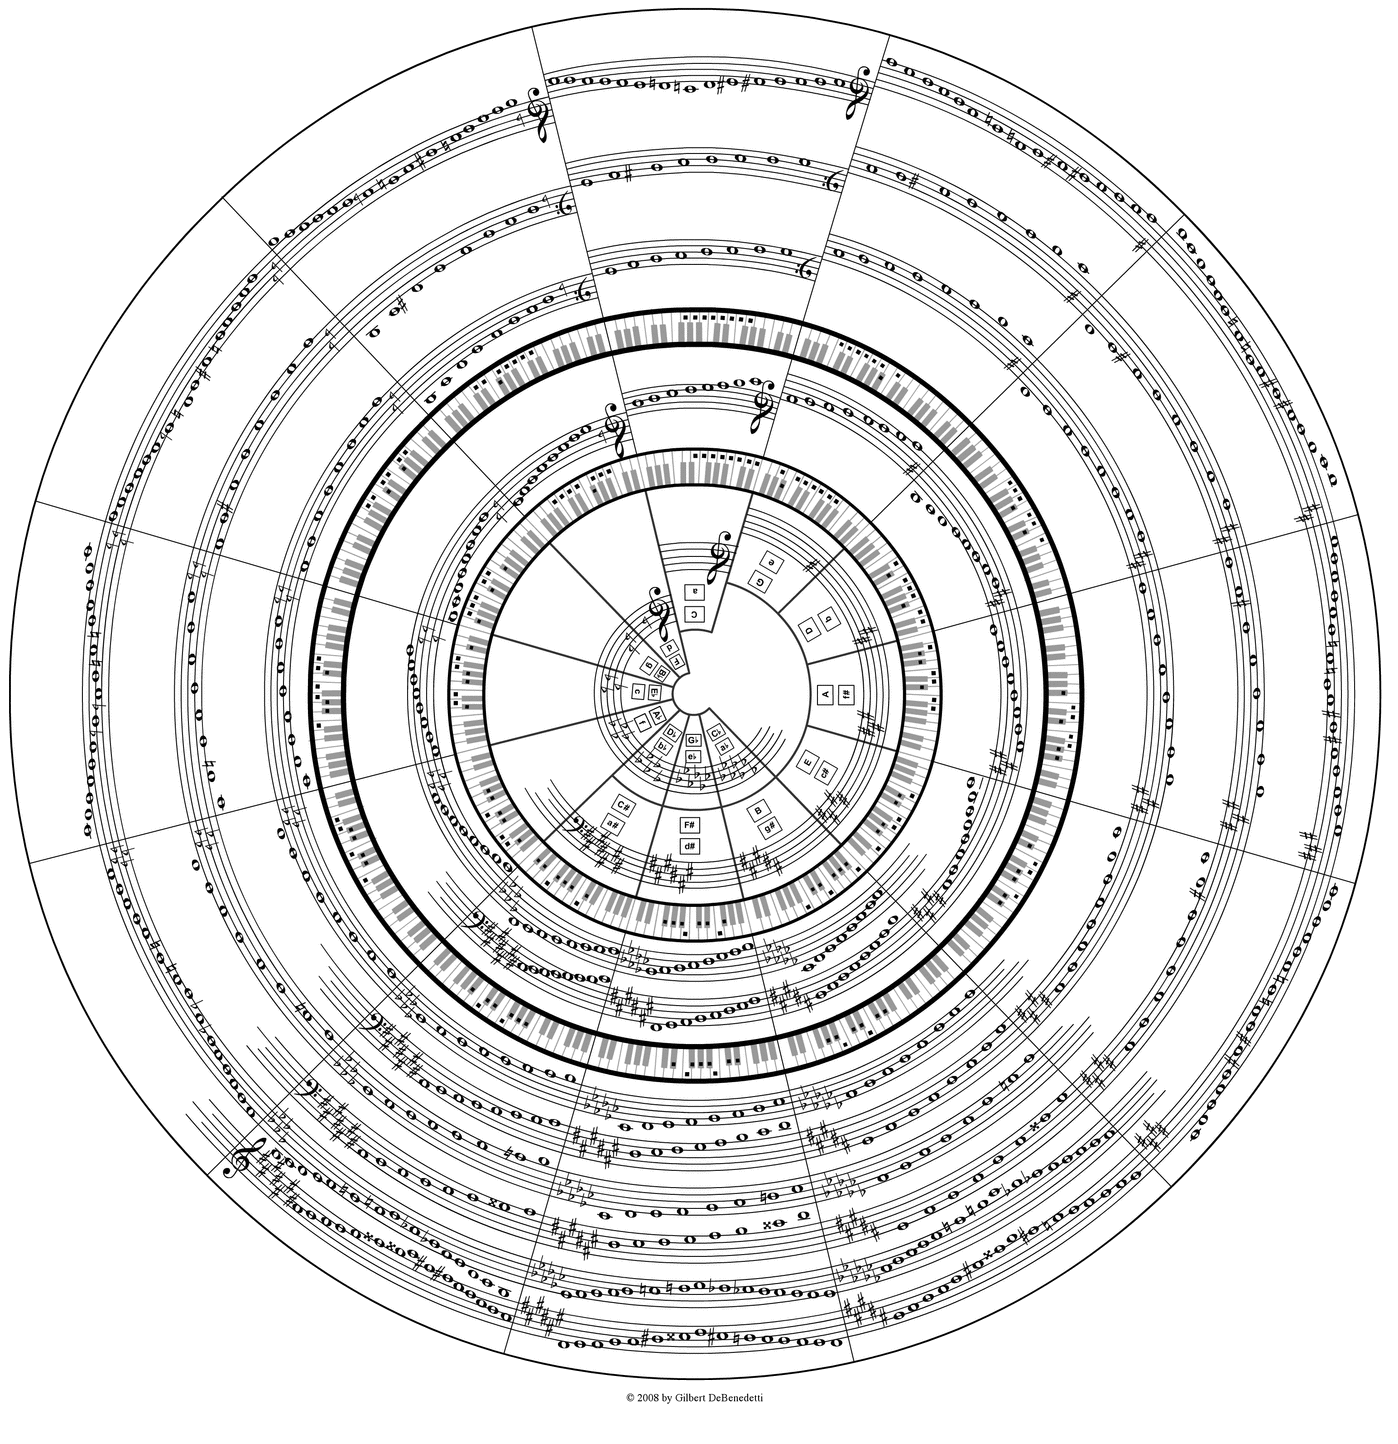
\includegraphics[width=.6\textwidth]{img/cover_img.png}~\\[2cm]

            % Author and supervisor
            \begin{minipage}{0.45\textwidth}
            \begin{flushleft} \large
                Rand ASSWAD\\
                Department of Applied Mathematics
            \end{flushleft}
            \end{minipage}
            \begin{minipage}{0.45\textwidth}
            \begin{flushright} \large
                \emph{Under the supervision of:}\\
                Prof. Natalie FORTIER
            \end{flushright}
            \end{minipage}

            \vfill
            % Bottom of the page
            {\large September 2021}
        \end{center}
    \end{sffamily}
\end{titlepage}
\makeatother

{
\setcounter{tocdepth}{3}
\tableofcontents
}
\def\R{\mathbb{R}}
\def\C{\mathbb{C}}
\def\N{\mathbb{N}}
\def\Z{\mathbb{Z}}

\def\x{\tilde{x}}
\def\w{\omega}
\def\phi{\varphi}

\def\dt{\mathrm{d}t}

\def\pp#1{\left(#1\right)}
\def\sset#1{\left\{#1\right\}}
\def\vset#1#2{\sset{#1\left\lvert#2\right.}}

\def\abs #1{\left\lvert#1\right\rvert}
\def\norm#1{\left\lVert#1\right\rVert}
\def\dotp#1#2{\left\langle#1{;}#2\right\rangle}

\def\pmat#1{\begin{pmatrix}#1\end{pmatrix}}

\def\qtext#1{\quad\text{#1}\quad}

\def\argmin{\mathop{\mathrm{argmin}}}
\def\argmax{\mathop{\mathrm{argmax}}}
\def\supp{\mathop{\mathrm{supp}}}

\def\transp#1{{#1}^{\top}}

\def\f{\boldsymbol{f}}
\def\ff{\f\hspace{-2pt}\f}
\def\mf{\boldsymbol{mf}}
\def\mp{\boldsymbol{mp}}
\def\p{\boldsymbol{p}}
\def\piu{pi\grave{u}~}

\def\X{\boldsymbol{X}}
\def\V{\boldsymbol{V}}
\def\W{\boldsymbol{W}}
\def\H{\boldsymbol{H}}

\pagebreak

\hypertarget{introduction}{%
\section*{Introduction}\label{introduction}}
\addcontentsline{toc}{section}{Introduction}

\pagebreak

\end{document}
